\section{Results}

\subsection{Automatic Evaluation}

Table~\ref{tab:main-results} reports failure-aware BGE-M3 cosine similarity and
BERTScore F1 for all four models across the three languages. All 142 samples
enter each mean; rows flagged as invalid (empty output, English copy, or
native-script corruption) receive zero for all metrics rather than being
excluded.

\begin{table}[t]
\centering
\small
\begin{tabular}{llrrr}
\toprule
Model & Language & BGE Cosine & BERT-F1 & Invalid \\
\midrule
\multirow{3}{*}{Anthropic} & Hindi   & 0.837 & 0.676 & 0 \\
                            & Telugu  & 0.789 & 0.671 & 4 \\
                            & Kannada & 0.733 & 0.620 & 5 \\
\midrule
\multirow{3}{*}{GPT-4o}    & Hindi   & 0.828 & 0.663 & 0 \\
                            & Telugu  & 0.794 & 0.667 & 0 \\
                            & Kannada & 0.749 & 0.641 & 2 \\
\midrule
\multirow{3}{*}{Gemini}    & Hindi   & 0.763 & 0.617 & 10 \\
                            & Telugu  & 0.630 & 0.548 & 25 \\
                            & Kannada & 0.664 & 0.569 & 19 \\
\midrule
\multirow{3}{*}{Ollama}    & Hindi   & 0.787 & 0.639 & 4  \\
                            & Telugu  & 0.598 & 0.574 & 16 \\
                            & Kannada & 0.537 & 0.549 & 20 \\
\bottomrule
\end{tabular}
\caption{Failure-aware automatic evaluation scores (response only). BGE Cosine
is BGE-M3 cosine similarity between the English reference and the romanized
output; BERT-F1 is raw multilingual BERTScore F1 using
\texttt{bert-base-multilingual-cased}. Invalid counts rows that received zero
(empty, English copy, or native-script corruption) out of 142 total.}
\label{tab:main-results}
\end{table}

\begin{figure}[t]
  \centering
  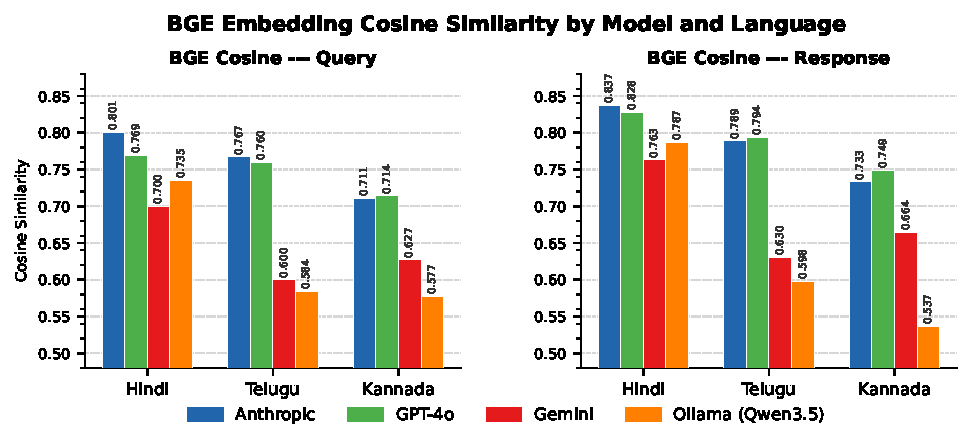
\includegraphics[width=\linewidth]{figures/bge_cosine.pdf}
  \caption{BGE-M3 cosine similarity for romanized queries (left) and responses
  (right) across all four models and three languages. Scores are failure-aware:
  empty, repeated, and script-corrupted outputs receive zero and are included in
  the mean over all 142 samples.}
  \label{fig:bge-cosine}
\end{figure}

\noindent{\sffamily\bfseries Language-level performance.}\enspace
Hindi obtains the highest scores across all four models (BGE: 0.763--0.837),
followed by Telugu (0.598--0.794) and Kannada (0.537--0.749). This ordering is
consistent with the availability of romanized Hindi training data: Hinglish is
the most widely represented romanized Indic variety in publicly available
corpora, while romanized Kannada and Telugu appear far less frequently.

\noindent{\sffamily\bfseries Model-level performance.}\enspace
Anthropic and GPT-4o produce the strongest and most reliable outputs. Both
achieve zero invalid rows for Hindi, and at most two for Telugu and Kannada.
Their BGE scores for Hindi (0.828--0.837) are the highest observed. Gemini and
Ollama degrade sharply on Telugu and Kannada, but for distinct reasons examined
in Section~\ref{sec:failures}.

\noindent{\sffamily\bfseries Misleadingly acceptable score range.}\enspace
A notable pattern is the narrowness of the BGE range for the two strongest
models: Anthropic and GPT-4o produce scores between 0.733 and 0.837 across all
language conditions. Considered in isolation, this band appears to indicate
acceptable semantic preservation. Section~\ref{sec:human-eval} shows that native
speakers do not agree.

\subsection{Failure Analysis}
\label{sec:failures}

Table~\ref{tab:failures} breaks down the two primary failure modes: responses
identical to the English source (repetition) and responses containing native
script characters (script corruption).

\begin{table}[t]
\centering
\small
\begin{tabular}{llrr}
\toprule
Model & Language & English-only & Script Spillage \\
\midrule
\multirow{3}{*}{Anthropic} & Hindi   & 0  & 0  \\
                            & Telugu  & 0  & 3  \\
                            & Kannada & 0  & 5  \\
\midrule
\multirow{3}{*}{GPT-4o}    & Hindi   & 0  & 0  \\
                            & Telugu  & 0  & 0  \\
                            & Kannada & 0  & 2  \\
\midrule
\multirow{3}{*}{Gemini}    & Hindi   & 0  & 8  \\
                            & Telugu  & 0  & 24 \\
                            & Kannada & 1  & 19 \\
\midrule
\multirow{3}{*}{Ollama}    & Hindi   & 3  & 0  \\
                            & Telugu  & 16 & 0  \\
                            & Kannada & 19 & 0  \\
\bottomrule
\end{tabular}
\caption{Failure breakdown per model and language (out of 142 rows). English-only
= response returned in English (word-overlap $\geq$ 0.90) instead of the
romanized target language. Script Spillage = response contains one or more
non-Latin characters (native script, Cyrillic, or other), after excluding
legitimate romanization diacritics (ā, ē, ṭ, etc.) and Catalan source-title
characters.}
\label{tab:failures}
\end{table}

Gemini and Ollama represent qualitatively different failure modes. Gemini
produces \emph{script spillage}: non-Latin characters appear mid-sentence in
otherwise romanized output. A detailed character-level scan of all responses
(after excluding legitimate romanization diacritics such as \={a}, \={e},
\d{t} and a Catalan source-title character in one play prompt) reveals that
spillage affects 24 of 142 Telugu responses (16.9\%), 19 of 142 Kannada
responses (13.4\%), and 8 of 142 Hindi responses (5.6\%) from Gemini. The
Telugu case is the most severe: Gemini produces entire paragraphs in native
Telugu script across 24 rows, totaling 2,635 Telugu characters. Anthropic
shows minor spillage confined to Kannada (5 rows) and Telugu (3 rows).
GPT-4o is nearly clean, with only 21 Kannada characters across 2 rows.
Ollama produces zero script spillage across all three languages.

Closer inspection reveals two unexpected spillage sub-types. First,
\emph{Cyrillic leakage}: Gemini Telugu row~53 inserts the Russian word
\emph{единственный} (``the only one'') into a mid-sentence position in an
otherwise Telugu-romanized narrative---an entirely non-Indic script appearing
in a Telugu romanization task. Anthropic Kannada also shows isolated Cyrillic
characters across 3 rows, unrelated to any Russian source content. Second,
\emph{cross-language script confusion}: Gemini's Kannada row~33 contains
Telugu script (\emph{అవును}) in a response that should be Kannada; Gemini's
Telugu row~19 simultaneously contains both Tamil script (\emph{சாத்தியம்}) and
Telugu script in the same line---two wrong scripts simultaneously. In Gemini
Hindi, script spillage takes a subtler form: the Devanagari word
\emph{मानना} (``believes'') recurs across 8 rows, left in native script
mid-Hinglish sentence rather than being romanized. These patterns suggest that
Gemini's script boundary is unstable in a way that standard automatic metrics
cannot detect: BGE-M3 and BERTScore measure semantic content, not whether the
output characters are in the correct script.

Ollama's dominant failure is \emph{English-only output}: the model returns the
answer in English instead of the romanized target language. Scanning all
$\sim$142 responses per model with a word-overlap threshold of $\geq$0.90
reveals 70 such instances in total. GPT-4o produces zero English-only outputs
across all three languages. Anthropic (10) and Gemini (9) cases are almost
entirely \emph{English-task rows}---prompts that operate on English text (OCR
cleanup, grammar correction, email improvement) where English output is
defensible; only $\sim$2 per model are genuine failures on prompts that
expected the target language. Ollama accounts for 51 instances, of which 41
are genuine failures on informational, creative, and conversational prompts.
English-only rates reach 14.7\% for Telugu and 30.4\% for Kannada, while
Hindi is largely unaffected at 2.8\%.

A second Ollama-specific failure is \emph{degeneration}: the model collapses
into repeating a single word or short phrase for hundreds to thousands of
tokens. We identify 13 such instances across the full dataset---every one
produced by Ollama, zero by any other model. The most extreme case is a Kannada
spelling-correction prompt where the word \emph{ellu} repeats 2,017
consecutive times across 2,020 total words. The automatic consistency check
(parameter P4 of our rubric) scores all 13 loops a perfect 3, and BGE-M3
assigns scores of 0.38--0.72---sometimes still ``passing.'' Human raters
assign usability zero to every degeneration case.

The two failure types do not overlap: Gemini never produces English-only output
and Ollama never leaks native script, suggesting the failures originate in
different aspects of instruction following. BERTScore and BGE-M3 treat both
failure types under the failure-aware policy: they receive zero. Without this
policy---if invalid rows were silently excluded---Gemini's Telugu BGE score
would rise from 0.630 to approximately 0.82, indistinguishable from GPT-4o's
0.794. The failure-aware denominator is therefore not cosmetic: it materially
changes model ranking.

\noindent{\sffamily\bfseries Why semantic metrics miss failures.}\enspace
A direct test of this blind spot is how automatic scores relate to English word
overlap. On the Ollama outputs, raw BERTScore-F1 correlates with English
word-overlap at $r = 0.955$ and BGE-M3 at $r = 0.805$: both metrics largely
reward how much of the output remains English rather than how well it is
romanized. Consistent with this, Ollama's verbatim-English Telugu responses
receive BGE $= 1.000$ and BERTScore-F1 $= 1.000$, while its genuine romanized
Telugu averages only $0.67$---the metric scores a complete task failure higher
than a success. Raw BERTScore-F1 is further compressed by a high floor: empty
responses still score ${\approx}0.42$, because baseline rescaling is disabled
and multilingual-BERT embeddings occupy a narrow cone. These properties explain
why the metric assigns its highest scores to its worst failures.

\begin{figure}[t]
  \centering
  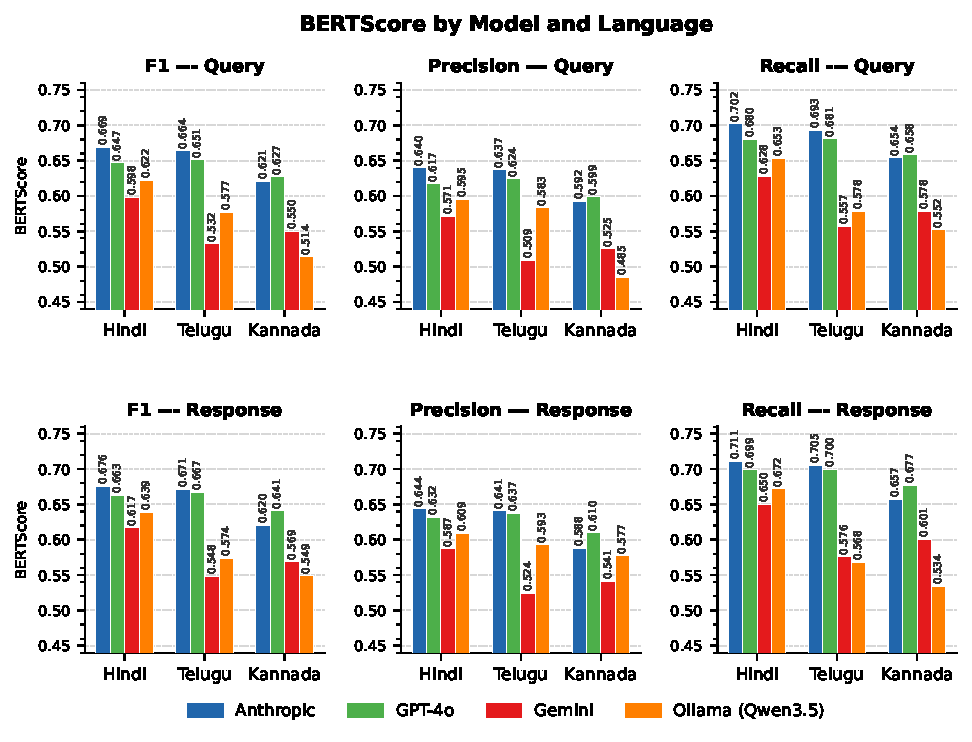
\includegraphics[width=\linewidth]{figures/bert_scores.pdf}
  \caption{Multilingual BERTScore (F1, Precision, Recall) for romanized queries
  (top row) and responses (bottom row) across all four models and three
  languages. Scores use \texttt{bert-base-multilingual-cased} and are
  failure-aware (invalid rows receive zero).}
  \label{fig:bert-scores}
\end{figure}

\subsection{Human Evaluation}
\label{sec:human-eval}

Automatic metrics operate on surface similarity. BGE-M3 computes cosine
distance between embedding vectors; BERTScore compares contextual token
representations. Both measure whether a romanized output is semantically close
to the English reference---but neither can answer the question that actually
matters: \emph{does this read like something a native speaker would type?}

Our automatic scores make the problem concrete. Across the two strongest
models, Anthropic and GPT-4o, BGE-M3 response scores span 0.733--0.837 across
all language conditions---a band that, considered in isolation, appears
acceptable. Yet automatic metrics cannot detect that a response uses the wrong
register, chooses a word that technically exists in the language but sounds
unnatural, or follows English sentence structure while using romanized
vocabulary. A model that produces grammatically correct but robotic-sounding
Hinglish receives the same score as one that sounds like a real person typing
on their phone.

Human evaluation targets precisely what BGE and BERTScore cannot see. Native
speakers of Hindi, Telugu, and Kannada rated approximately 24 responses per
language (73 total) across all four models on five dimensions: naturalness and
fluency, grammatical correctness, word choice accuracy, register
appropriateness, and overall usability (each on a 2--3 point scale; maximum
12 points per response). Rows were selected to include metric-disagreement
cases (where BGE and BERTScore diverge by more than 0.15 points), hard
narrative prompts, and failure anchors---precisely the cases where automatic
metrics are most likely to miss real quality differences.

\noindent{\sffamily\bfseries Annotation procedure.}\enspace
To accelerate review without sacrificing quality, we first generated reference
scores for all ten parameters using Claude Opus 4.8 as an LLM judge. Native
speakers then received pre-filled sheets and were instructed to correct any
value they disagreed with, reading each \texttt{romanized\_response} before
accepting or overriding the draft score. The final H6--H10 scores are native-speaker judgments where a reviewer has
corrected the draft; uncorrected rows remain at the LLM-judge value. To gauge
whether the LLM judge can stand in for native speakers, a native reader
re-scored a blind sample of Telugu rows. Agreement is poor: although the mean
signed difference is near zero, this masks a mean absolute deviation of roughly
4 points out of 12, because the judge errs in opposite directions that cancel.
It over-rates genuine failures---one Gemini Telugu response containing
native-script characters and a stray Russian word received 10.4/12 from the
judge but 3/12 from the native reader---and under-rates legitimate
English-task outputs, which it penalizes for not being in the target language.
The LLM judge is therefore subject to the same blindness as the embedding
metrics, and we treat native judgments, not the judge, as ground truth. Hindi
scores are LLM-judge reference values pending native-speaker review and should
be treated as provisional. Telugu and Kannada scores reflect native-speaker
corrections applied over the LLM-judge draft. Whether an LLM judge can
reliably substitute for native speakers on romanized Indic evaluation is itself
a finding we return to in Section~\ref{sec:discussion}.

\begin{table}[t]
\centering
\small
\begin{tabular}{lrrrrrrr}
\toprule
Model & Nat. & Gram. & Word & Reg. & Usab. & Total & BGE \\
      & /3   & /2    & /2   & /2   & /3    & /12   & (ref) \\
\midrule
GPT-4o    & 2.49 & 1.93 & 1.97 & 1.94 & 2.40 & \textbf{10.73} & 0.790 \\
Anthropic & 2.05 & 1.66 & 1.70 & 1.73 & 2.15 & 9.30  & 0.786 \\
Gemini    & 1.89 & 1.73 & 1.54 & 1.70 & 2.06 & 8.91  & 0.686 \\
Ollama    & 0.76 & 0.89 & 0.93 & 1.04 & 0.85 & 4.48  & 0.641 \\
\bottomrule
\end{tabular}
\caption{Human-corrected LLM-judge scores (weighted mean across all languages,
73 total rows: $\sim$24 per language). Telugu and Kannada rows have
native-speaker corrections applied over the LLM-judge draft; Hindi scores are
LLM-judge reference values (provisional, pending native-speaker review).
Nat.=Naturalness/Fluency, Gram.=Grammar Correctness, Word=Word Choice
Accuracy, Reg.=Register Appropriateness, Usab.=Overall Usability. BGE column
shows mean failure-aware BGE-M3 response score from
Table~\ref{tab:main-results} for reference.}
\label{tab:human-eval}
\end{table}

\noindent{\sffamily\bfseries Metric--human disagreement.}\enspace
Table~\ref{tab:human-eval} exposes the central finding of this paper.
BGE-M3 scores for Anthropic (0.786) and GPT-4o (0.790) are nearly
indistinguishable---a difference of 0.004 points that no downstream decision
would act on. Native speakers disagree sharply: GPT-4o scores 10.73 out of 12
while Anthropic scores 9.30, a gap of 1.43 points driven primarily by
naturalness (2.49 vs 2.05) and register appropriateness (1.94 vs 1.73). The
metric ranking and the human ranking disagree at the top.

The gap is most severe for Ollama. BGE-M3 assigns it 0.641---poor, but not
catastrophic by the metric's scale. Human raters assign a mean of 4.48 out of
12, with Telugu and Kannada responses averaging 4.07 and 2.86 respectively
(largely unusable), while Hindi averages 8.28---a divergence explained by
Ollama's near-complete instruction collapse in Dravidian languages (30\% of
Kannada outputs returned in English) versus better Hindi coverage in its
training data. BGE cannot distinguish between a response that is semantically
adjacent but linguistically broken and one that is simply the English source
returned verbatim---both score near 1.000 under that policy. Human raters make
this distinction immediately.

\noindent{\sffamily\bfseries Language and register effects.}\enspace
Human scores follow the same language ordering as automatic metrics: Hindi
obtains the highest mean (9.42/12, provisional---LLM-judge scores pending
native-speaker review), followed by Kannada (7.11/12) and Telugu (6.89/12).
The Hindi figure should be treated with caution as it has not yet been
corrected by a native speaker, unlike the Telugu and Kannada scores which
reflect direct native-speaker judgments. Register appropriateness is the most
commonly flagged failure dimension in evaluator notes: Gemini responses in all
three languages were described as ``too formal'' or using ``very formal words''
inconsistent with the conversational register of the prompts. One GPT-4o
Kannada response was noted as ``almost English''---a high-overlap output that
BGE would score near 1.0 but that native speakers identified as a task failure.

\noindent{\sffamily\bfseries Overall comparison.}\enspace
Table~\ref{tab:summary} consolidates automatic and human evaluation results
across all models. The contrast between automatic and human ranking is the
central finding: BGE-M3 separates Anthropic and GPT-4o by only 0.004 points,
while human raters assign them a 1.43-point gap. Ollama receives a BGE score
of 0.641---below the other models but still within a plausible range---yet
human raters score it 4.48 out of 12, less than half the score of any other
model.

\begin{table}[t]
\centering
\small
\begin{tabular}{lrrrr}
\toprule
Model & BGE-M3 & BERT-F1 & Human /12 & English-only \\
      & (mean) & (mean)  & (mean)    & failures \\
\midrule
GPT-4o    & \textbf{0.790} & \textbf{0.657} & \textbf{10.73} & 0  \\
Anthropic & 0.786          & 0.656          & 9.30           & 2  \\
Gemini    & 0.686          & 0.578          & 8.91           & 2  \\
Ollama    & 0.641          & 0.587          & 4.48           & 41 \\
\bottomrule
\end{tabular}
\caption{Summary of all evaluation results. BGE-M3 and BERT-F1 are
failure-aware means over all 142 responses per model (averaged across
languages). Human /12 is the weighted mean human score across 73 evaluated
rows ($\sim$24 per language; Hindi provisional). English-only failures are
genuine cases (excluding English-task prompts) where the model returned
English instead of the romanized target language, counted over the full
$\sim$142-response set. GPT-4o is the only model with zero English-only
failures across all three languages.}
\label{tab:summary}
\end{table}
